Tunnistimme aineistostamme eri oppilastyyppejä.
Kaikki haastatellut oppilaat pitivät harjoituskurssia hyödyllisenä.
Syyt kuitenkin vaihtelivat; suuri osa ($n=9$) piti kurssia hyödyllisenä sen kertaavan luonteen vuoksi.
Neljän opiskelijan mielestä kurssilla on opittu myös uusia asioita, muun muassa laskimen käyttötaitoa.
Kuusi opiskelijaa ei vastannut kysymykseen.
Hyvänä ominaisuutena pidettiin myös sitä, että apua ja neuvontaa on saatavilla.

\begin{figure}[h!]
\centering
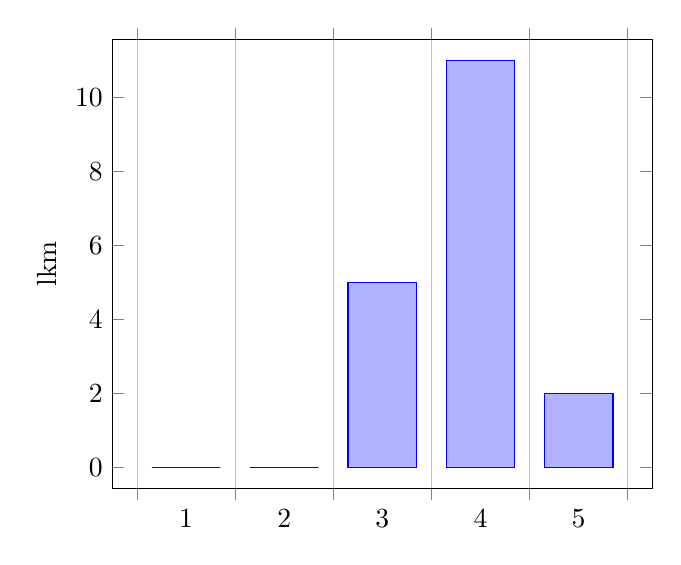
\begin{tikzpicture}
\begin{axis}[x tick label 
style={/pgf/number format/1000 sep=}, ylabel=lkm, enlargelimits=0.05, legend style={at={(0.5,-0.15)}, anchor=north,legend columns=-1},ybar interval=0.7]
\addplot coordinates {(1,0) (2,0) (3,5) (4,11) (5,2) (6,0)}; % miksei piirrä vikaa asiaa? :3
\end{axis}
\end{tikzpicture}
\caption{``Harjoituskurssista on ollut minulle hyötyä.''}
\end{figure}

\subsection{Kisälliopetus}
Kurssi toteuttaa kisälliopetuksen piirteet opiskelijoiden vastauksien mukaan hyvin.
Suurin osa opiskelijoista ($n=12$) kiitteli vastauksissaan sitä, että apua on saatavilla hyvin.
Loput ($n=7$) opiskelijat eivät kommentoineet vastausta, mutta olivat jokseenkin samaa mieltä tai täysin samaa mieltä siitä, että kurssilla saa apua hyvin.

\begin{figure}[h!]
\centering
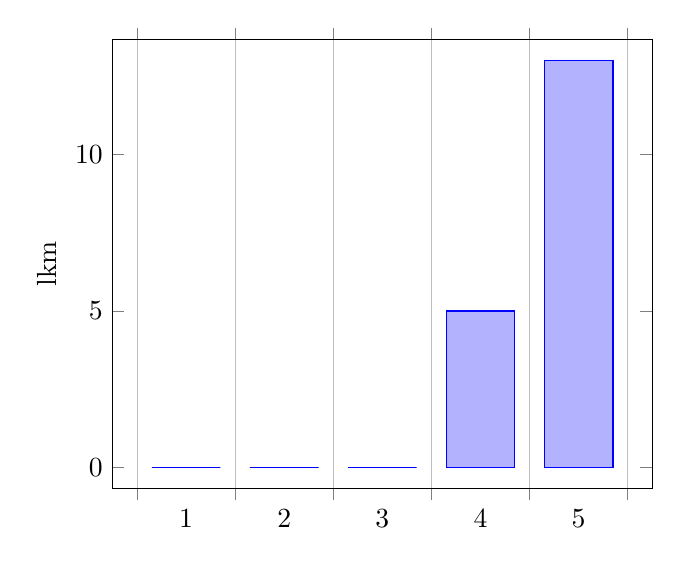
\begin{tikzpicture}
\begin{axis}[x tick label 
style={/pgf/number format/1000 sep=}, ylabel=lkm, enlargelimits=0.05, legend style={at={(0.5,-0.15)}, anchor=north,legend columns=-1},ybar interval=0.7]
\addplot coordinates {(1,0) (2,0) (3,0) (4,5) (5,13) (6,0)}; % miksei piirrä vikaa asiaa? :3
\end{axis}
\end{tikzpicture}
\caption{``Saan harjoituskurssilla apua tehtävien ratkaisemiseen.''}
\end{figure}

Myös \emph{scaffolding}-ilmiö esiintyy vastauksissa.

\begin{figure}[h!]
\centering
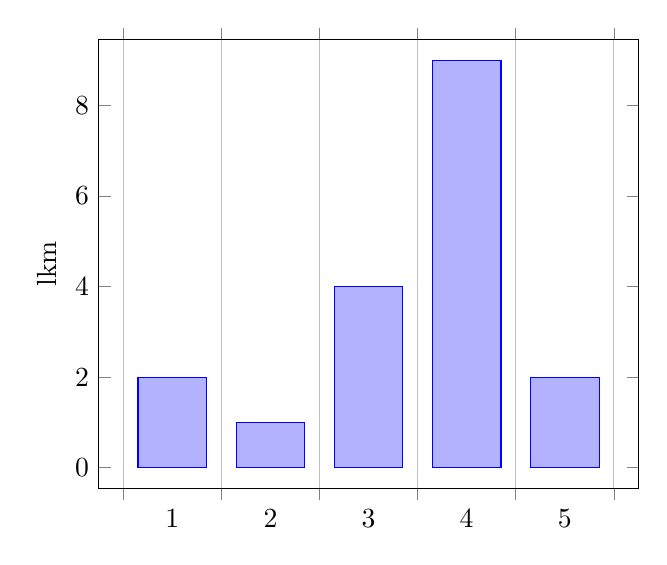
\begin{tikzpicture}
\begin{axis}[x tick label 
style={/pgf/number format/1000 sep=}, ylabel=lkm, enlargelimits=0.05, legend style={at={(0.5,-0.15)}, anchor=north,legend columns=-1},ybar interval=0.7]
\addplot coordinates {(1,2) (2,1) (3,4) (4,9) (5,2) (6,0)}; % miksei piirrä vikaa asiaa? :3
\end{axis}
\end{tikzpicture}
\caption{``Saan harjoituskurssilla tehtyä sellaisiakin tehtäviä, joita en itsenäisesti osaisi tehdä.''}
\end{figure}

Itsevarmuus omasta osaamisesta vaikuttaa opiskelijan matematiikkapelkoon.
Se, että opiskelija kokee korkeaa minäpystyvyyden tunnetta on myös välttämätöntä \emph{flow}-tilaan pääsemiseksi.
%Vastauksista voi myös päätellä, että harjoituskurssi torjuu opiskelijoiden matematiikkapelkoa.

\begin{figure}[h!]
\centering
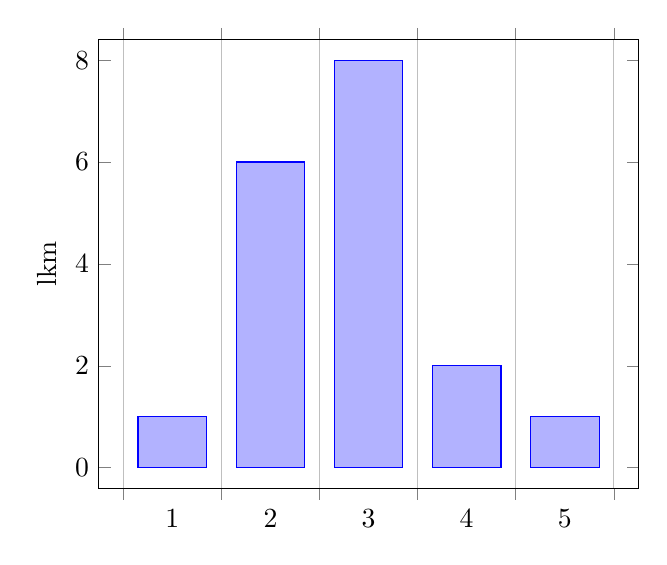
\begin{tikzpicture}
\begin{axis}[x tick label 
style={/pgf/number format/1000 sep=}, ylabel=lkm, enlargelimits=0.05, legend style={at={(0.5,-0.15)}, anchor=north,legend columns=-1},ybar interval=0.7]
\addplot coordinates {(1,1) (2,6) (3,8) (4,2) (5,1) (6,0)};
\end{axis}
\end{tikzpicture}
\caption{``Harjoituskurssi on lisännyt itsevarmuuttani matematiikan osaamisen suhteen.''}
\end{figure}

Opiskelijat, jotka olivat täysin tai jokseenkin eri mieltä väitteen kanssa vastasivat muun muassa, että itsevarmuus riippuu vain käsiteltävien aiheiden mielekkyydestä, että yksi kurssi ei riitä itsevarmuuden kehittämiseen ja että itsevarmuutta vähentää se, että ei saa helpoksi luonnehdittua tehtävää ratkaistua.


\subsection{Opiskelijoiden matematiikkakuva}
Kyselyvastauksista kävi ilmi, että moni opiskelija pitää matematiikkaa enimmäkseen laskemisena.
Lisäksi matemaattisen taidon koetaan kehittyvän harjoittelun avulla.


\subsection{Kurssin vaativuustaso}
Osalle opiskelijoista kurssi oli sopivan vaativa, mutta monet kokivat myös tylsistyvänsä tunnilla.
Tämä tarjoaisi hedelmällisen mahdollisuuden eriyttää opetusta; jos tehtävämonisteita olisi kaksi, kertaava ja syventävä, kurssi palvelisi laajempaa opiskelijajoukkoa.
Koska kurssisuoritukseen riittää vain läsnäolo, valmistaa kurssi myös korkeakoulujen akateemiseen vapauteen; opiskelijalla on vastuu omasta työskentelystään.
Tämä saattaa lisäksi hillitä matematiikkapelkoa, sillä opiskelijalla ei ole paineita suorittaa tiettyä määrää tehtävistä.

\subsection{Miten kurssia voisi kehittää?}



